\documentclass[12pt]{article}

\usepackage[margin=1in]{geometry}
\usepackage[utf8]{inputenc}
\usepackage[T1]{fontenc}
\usepackage{lmodern}
\usepackage{microtype}
\usepackage{setspace}
\usepackage{parskip}
\usepackage{url}
\usepackage{booktabs}
\usepackage{threeparttable}
\usepackage[font={footnotesize}]{caption}
\usepackage{float}
\usepackage{graphicx}
\usepackage{lscape}
\usepackage[super,comma,sort&compress]{natbib}
\bibliographystyle{unsrtnat}
\usepackage[colorlinks=true, urlcolor=blue, linkcolor=black, citecolor=black]{hyperref}

% Auto-generated by code/generate_faq_numbers.R. Do not edit by hand.
\newcommand{\faqNovelty}{1}
\newcommand{\faqProvision}{2}
\newcommand{\faqInsurance}{3}
\newcommand{\faqPharma}{4}
\newcommand{\faqPriceFixing}{5}
\newcommand{\faqCentralPlanning}{6}
\newcommand{\faqBundles}{7}
\newcommand{\faqNegotiatorPay}{8}
\newcommand{\faqFines}{9}
\newcommand{\faqOptOut}{10}
\newcommand{\faqRural}{11}
\newcommand{\faqWithdrawal}{12}
\newcommand{\faqInnovation}{13}
\newcommand{\faqFiscal}{14}


% Allow figures and tables to float more freely: let them take up most of a page
% if needed, and do not leave large gaps chasing a perfect placement.
\renewcommand{\topfraction}{0.9}
\renewcommand{\bottomfraction}{0.8}
\renewcommand{\textfraction}{0.07}
\renewcommand{\floatpagefraction}{0.7}
\setcounter{topnumber}{3}
\setcounter{bottomnumber}{3}
\setcounter{totalnumber}{5}

\onehalfspacing

\title{One Drug, Many Prices:\\A Proposal to Reform US Healthcare Pricing}
\author{}
\date{}

\begin{document}

\maketitle
\thispagestyle{empty}

\subsection*{Introduction}

The US healthcare pricing system is broken: the same product is sold to different payers for wildly different amounts, patients cannot compare or even know the price of their care beforehand, pharmacy benefit managers coerce payment of undisclosed sums for themselves and hide the amounts as a tightly guarded secret, and the largest public insurer is effectively barred from using its leverage to reduce prices.

I propose three reforms: consolidated government negotiation, Bloc-wide pricing as a condition of market access, and a central price lookup system. Each has been tried or proposed in isolation. The contribution of this note is to show how the three complement one another, with each closing a loophole the others leave open (see \href{https://rabbanimaysam.github.io/health-reform-proposal/faq.html}{FAQ \faqNovelty}).

Figure~\ref{fig:pricegaps} shows the payment gap across ten commonly used drugs, hospital services, and outpatient procedures. For example, a colonoscopy costs \$880 at the VA, \$1,760 under Medicare, \$5,816 under a commercial insurer, and \$19,206 for uninsured patients. This is not an anomaly. In every case, the price of the same product or service swings several-fold across payers, and in every case the uninsured, the most vulnerable group, pay the most.

\begin{figure}[htbp]
\centering
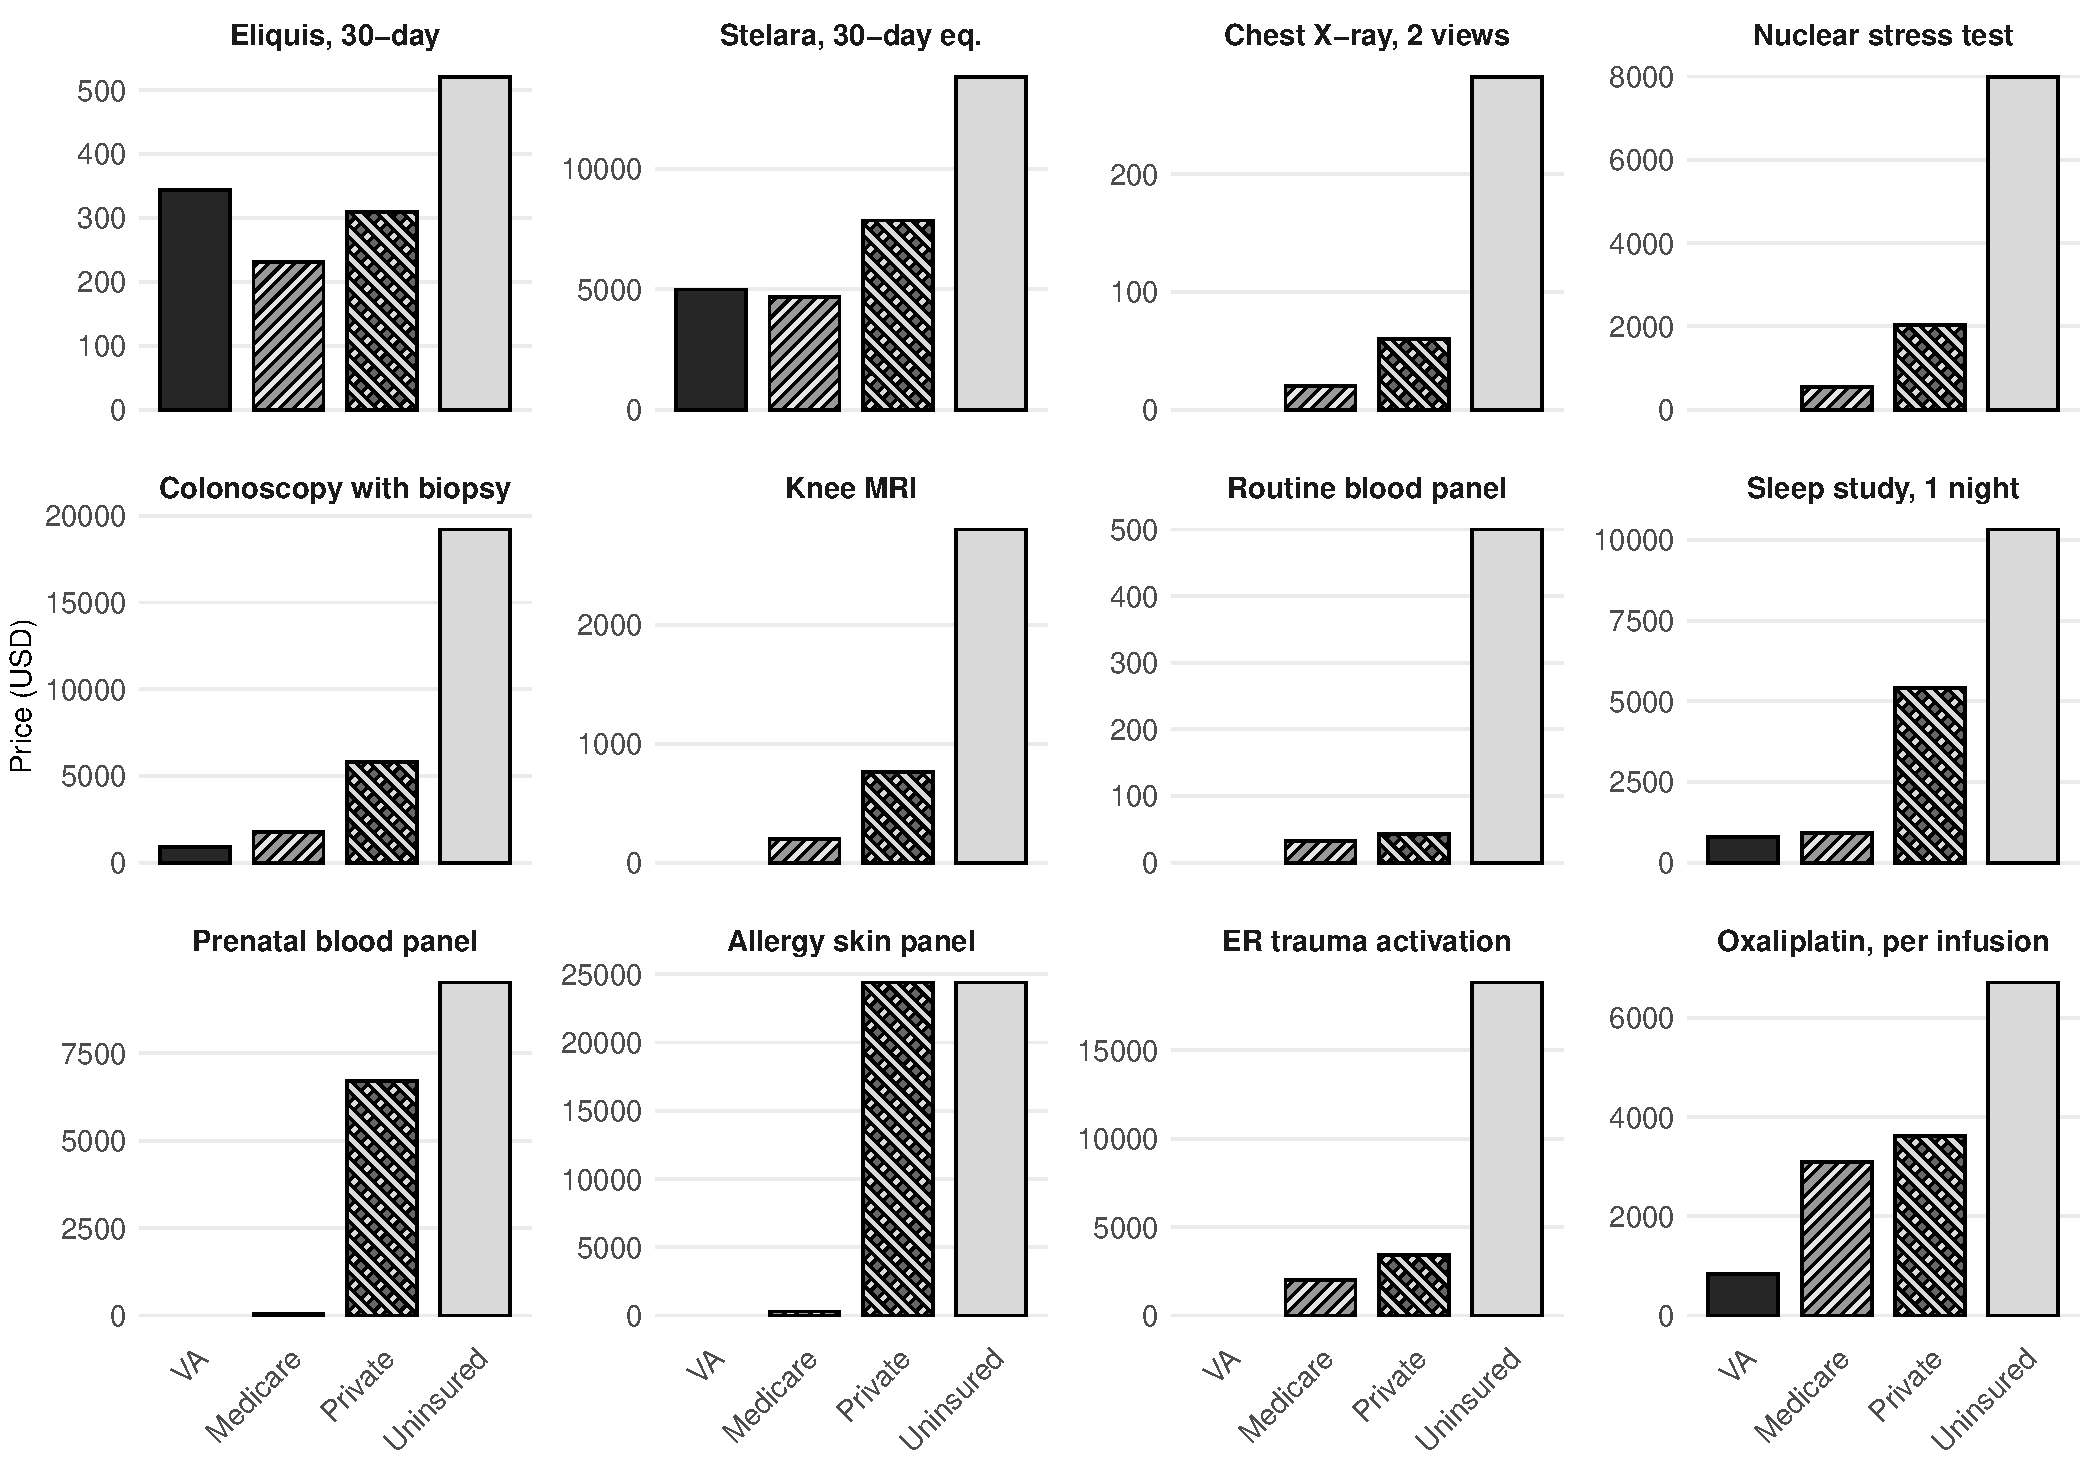
\includegraphics[width=0.9\textwidth]{fig_pricegaps.pdf}
\caption{Price gaps across payers for the same service or product.}
\label{fig:pricegaps}
\vspace{2pt}
\begin{minipage}{\textwidth}
\fontsize{8}{9}\selectfont
\textit{Notes:} The "private insurer" bar is the total negotiated rate, including patient cost-sharing; the "uninsured" bar is the chargemaster or list price. Each panel uses its own vertical scale. Missing bars indicate that a reliable figure was not available in the cited sources. Full sources and derivations are on the \href{https://rabbanimaysam.github.io/health-reform-proposal/price-gaps.html}{companion site}.
\end{minipage}
\end{figure}

Americans usually do not know the price at the time of receiving care, and this opacity is a key driver of the price dispersion shown above. The secrecy is structural. No other developed nation operates a pricing system this opaque.

Two forces determine an insurer's ability to bring down prices: its size, and the availability of alternatives. A large insurer has more leverage because losing its volume hurts providers more, but if providers can walk to another insurer offering higher rates, that leverage evaporates. Leverage is maximized when the insurer is both large and difficult to replace. The three reforms below are designed around this logic. Consolidated negotiation makes the government a single, large insurer. Bloc-wide pricing eliminates the alternatives that providers could otherwise turn to for higher rates. A central price lookup system ensures the negotiated prices are honored, not undercut by secret side deals.

\subsection*{Reform 1: Consolidated government negotiation}

The federal government does not negotiate healthcare prices as a single insurer. It fragments its purchasing power across Medicare, Medicaid, and at least nine other programs, each with its own formulary, fee schedule, rules, and leverage. For prescription drugs alone, these programs account for 51\% of US spending, yet they compete against one another instead of bargaining as one.\citep{cms2024nhe} Hospital and physician payments are just as fragmented. Consolidating these programs into a single negotiating Bloc would use leverage the government has but wastes. Other developed nations leverage their full size in what resembles a bloc, and pay far less.\citep{gusmano2020price}

For most of its history, Medicare was statutorily prohibited from negotiating drug prices, a restriction unparalleled in the developed world. The Inflation Reduction Act of 2022 began to reverse it, authorizing Medicare to negotiate prices for ten high-expenditure drugs. Figure~\ref{fig:intlprices} compares prices in the US and six other developed countries for nine of those ten drugs. The US list price towers over what every peer nation pays. Even after rebates and discounts, private insurers in the US pay multiples of what patients in Canada, France, or the UK pay for the same drug. Medicare's newly negotiated prices narrow the gap but remain well above the rest of the developed world, cutting net prices by roughly 22\% on average, with reductions reaching beyond 30\% on the highest-cost drugs.\citep{kff2024ira} Confining negotiation to ten drugs squanders the government's broader leverage. The VA, by contrast, is not prohibited from negotiating, and despite its much smaller size pays roughly half of what Medicare Part D pays.\citep{cbo2022commercial, cbo2021drugprices, gao2021vadrugs}

\begin{figure}[htbp]
\centering
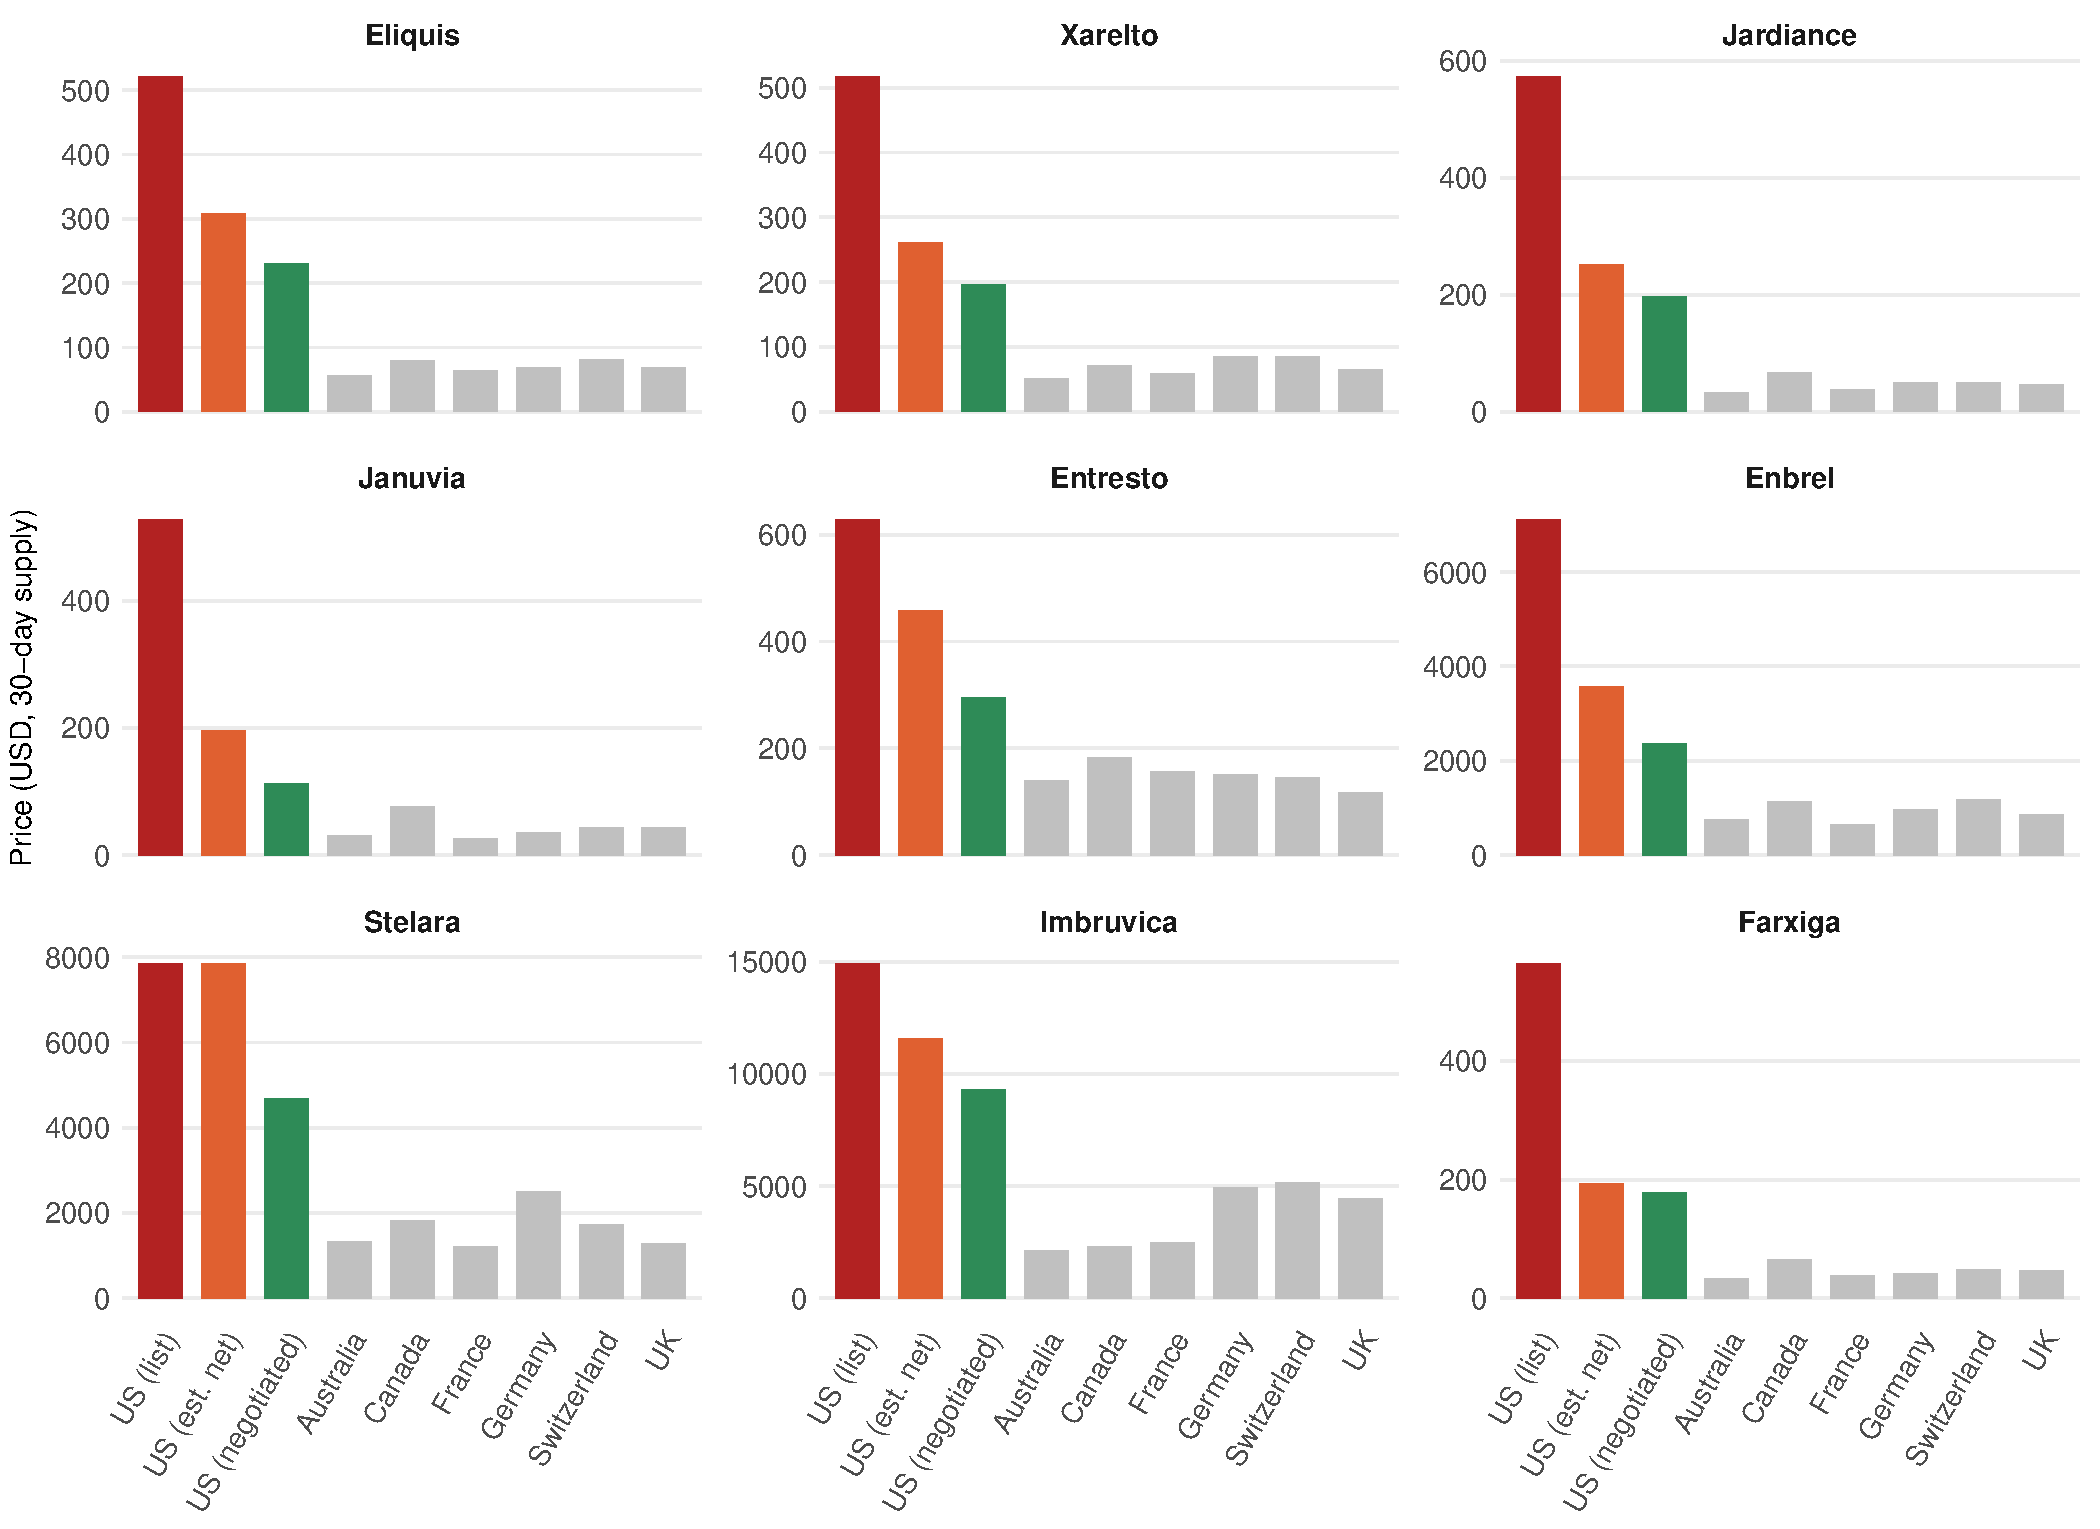
\includegraphics[width=\textwidth]{fig_intlprices.pdf}
\caption{Drug prices by country.}
\label{fig:intlprices}
\vspace{2pt}
\begin{minipage}{\textwidth}
\fontsize{8}{9}\selectfont
\textit{Notes:} The solid dark bar is the US list price (paid by the uninsured). The striped bar is the estimated US net price across all US payers combined, after rebates and discounts, derived from SSR Health data and SEC filings.\citep{wouters2025jama} The crosshatched bar is the Medicare negotiated price under the Inflation Reduction Act (effective 2026). Insulin aspart is excluded due to reporting incompatibility across countries. Each panel uses its own vertical scale. Full figures and sources are on the \href{https://rabbanimaysam.github.io/health-reform-proposal/international-prices.html}{companion site}.
\end{minipage}
\end{figure}

Reform 1 outlaws rebates, chargebacks, spread pricing, and side payments of any kind. Negotiation is conducted by salaried Bloc negotiators with expertise in pharmacology, clinical medicine, and health economics, who also make formulary and tiering decisions. Bloc negotiators are prohibited from accepting any payment beyond their government compensation package, and for twelve months after leaving the Bloc are barred from employment in any sector of the regulated healthcare industry. Compensation follows the federal Senior Executive Service model: a fixed salary at the SES level and a performance bonus capped at 10\% of base, awarded on periodic peer-reviewed evaluations rather than per-contract outcomes (see \href{https://rabbanimaysam.github.io/health-reform-proposal/faq.html}{FAQ \faqNegotiatorPay}).

Smaller-scale precedents exist. The Federal Supply Schedule publishes VA-negotiated contract prices that the Department of Defense (including Tricare), the Indian Health Service, the Federal Bureau of Prisons, and the Public Health Service all purchase off,\citep{vafss2026} demonstrating that one negotiating body can serve many federal agencies at a single negotiated price. At the state level, pooled purchasing coalitions such as the Sovereign States Drug Consortium extract supplemental Medicaid rebates of 5 to 15\% beyond federal levels by combining state purchasing power.\citep{oig2014supplementalrebates, horvath2019purchasing}

In short, Reform 1 is to pool all federal healthcare purchasing into one Bloc that negotiates prices for every covered drug, hospital service, and physician service on behalf of every federal program.

\subsection*{Reform 2: Bloc-wide pricing as a condition of market access}

Any provider that contracts with the Bloc retains the freedom to choose which private insurers to contract with, but once a contract is signed, the price must be the same as the Bloc-negotiated rate. Uninsured patients cannot be refused or charged a different price. The negotiated price is locked in: no insurer can negotiate further discounts on the side. Any provider that violates these terms loses its contract with the Bloc, and with it, access to the majority of the market.

Reform 2 does not make insurance plans identical; it standardizes the price, not the coverage. Once the price of a service is fixed, insurers would compete on what fraction of that price they cover and what fraction the patient pays out of pocket. Generous plans would leave the patient with a small copay; cheaper plans would expose patients to more. Both would pay the provider the same.

The logic of all-payer pricing has been defended in the US health-policy literature for decades, most prominently by Reinhardt,\citep{reinhardt2011allpayer} and Maryland has operated an all-payer hospital system since 1977. Conditioning federal market access on pricing is also well-established: the 340B Drug Pricing Program requires manufacturers in Medicaid to sell to safety-net providers at roughly 25 to 50\% below list, and the Medicaid Best Price rule requires manufacturers to offer Medicaid the lowest price offered to any non-federal purchaser. Reform 2 combines the all-payer tradition with the conditional-access enforcement tool.

\subsection*{Reform 3: A central price lookup system}

Reforms 1 and 2 produce one negotiated price per provider per service. Reform 3 makes that price visible. The Bloc operates a public price lookup system, the canonical record of every contracted price in the country. Each entry pairs a service code with a provider and a price. It updates whenever a contract is signed or revised.

Every Bloc contract pre-sets the price of every covered service, whether per service or per bundled episode. Bloc officials transfer those prices from the contract to the database directly, with no provider input. This sidesteps the misreporting, gaming, and non-compliance that become systemic whenever transparency depends on thousands of providers posting their own data.

The lookup system is open, free, and built for comparison. Patients can compare providers within a chosen radius before scheduling care, and physicians, who are more informed and more influential in directing demand, can route patients to lower-priced providers when prescribing or referring. A public API lets third parties integrate prices into comparison tools, electronic health records, and patient portals.

Price transparency is a known driver of price reductions (see \href{https://rabbanimaysam.github.io/health-reform-proposal/faq.html}{FAQ \faqNovelty}), but only if the posted prices are the actual prices and if transparency is enforced. Existing federal transparency rules have failed on both counts: they require posting in formats too inconsistent to compare, and punish non-compliance with symbolic penalties. Under the proposed reform, the Bloc posts actual contracted prices, and any patient charged more than the listed price can file a complaint. Deterrence requires large fines, for example a multiplier on the order of 100 times the overcharge (see \href{https://rabbanimaysam.github.io/health-reform-proposal/faq.html}{FAQ \faqFines}), and contract termination for repeat offenders.

\subsection*{Final word}

Patients would be the biggest beneficiaries of these reforms. They would pay less, comparison-shop among providers, and know the price before receiving care. Insured patients would see lower premiums as the prices underlying them fall, and uninsured patients, who face the highest prices in today's system, would pay the same listed price as everyone else. The US pays multiples of what every other developed country pays for the same drugs, services, and procedures, for no reason more defensible than institutional inertia. The tools to change that are not exotic. They are familiar, tested at smaller scales, and in partial use across the federal healthcare system. What is missing is the decision to put them together.

The \href{https://rabbanimaysam.github.io/health-reform-proposal/faq.html}{online FAQ} answers a set of common questions about the proposal. Comments, criticisms, and suggestions are welcome through \href{https://rabbanimaysam.github.io/health-reform-proposal/}{this link}.

{\scriptsize
\setlength{\bibsep}{0pt}
\bibliography{references}
}

\end{document}
